%%%%%%%%%%%%%%%%%%%%%%%%%%%%%%%%%%%%%%%%%
%%%%%%%%%% Content starts here %%%%%%%%%%
%%%%%%%%%%%%%%%%%%%%%%%%%%%%%%%%%%%%%%%%%

\begin{frame}{Overview}
	\begin{itemize}[<+-| alert@+>]
	  \item What is E-Lab?
	  \item Motivation
	  \item The problems
	  \item The solution
	  \item E-Lab philosophy
	  \item Architecture
	  \item Conclusion
	\end{itemize}
\end{frame}


\begin{frame}{What is E-Lab?}
	\begin{itemize}[<+-| alert@+>]
	  \item \emph{E-Lab} is a system for solving and auto-grading programming
	  problems from introduction programming courses
	  \item Everything is done in a web browser
	  \item Using the power of version control systems
	  \item Sandboxed execution
	  \item Supporting different types of problems in several programming languages
	  (C, C++, Java)
	  \item Designed for scalability and extension
	\end{itemize}
\end{frame}

\begin{frame}{Motivation}
	\begin{itemize}[<+-| alert@+>]
	  \item Programming is one of the essential practical skills in computer science curriculums
	  \item Great popularity among high school students resulting in large
	  introduction classes with several hundreds of students enrolled
	  \item But programming is not easy!
	  \item Involves solving a lot of basic algorithmic examples (1/3 of the time)
	\end{itemize}
\end{frame}

\begin{frame}{The problems}
	\begin{itemize}[<+-| alert@+>]
	  \item The context
	  \begin{itemize}
	  	\item X * 100 students
	  	\item Divided in groups up to 20
	  	\item 3 - 6 problems a week
		\end{itemize}
		\item The problems
	  \begin{itemize}
	  \item Each  instructor should examine and assess up to 120 solutions in 15
	  minutes
	  \item Students' feedback
	  \item Loosing focus from the actual programming
	 \end{itemize}
	\end{itemize}
\end{frame}

% Define block styles
\tikzstyle{block} = [rectangle, draw, fill=blue!20,
text width=5em, text centered, rounded corners, minimum height=4em]
\tikzstyle{line} = [draw, -latex']

\begin{frame}[fragile]{The solution}
	\begin{itemize}
  	  \item Algorithmic type of problems 
	\end{itemize}
\begin{center}
\begin{tikzpicture}[node distance = 3cm, auto]
    % Place nodes
    \pause
    \node [block] (input) {Input};
    \pause     
    \path [line] (input) -> node {} (algorithm);
    \node [block, right of=input] (algorithm) {Algorithm}
    \pause
    \path [line] (algorithm) -> node {} (output);
    \node [block, right of=algorithm] (output) {Output};
    % Draw edges
\end{tikzpicture}
\end{center}
\pause
\begin{itemize}[<+->]
  \item Used in competitive programming systems
  \item Importance in programming to have working solution 
\end{itemize}
\end{frame}

\begin{frame}{E-Lab Goals}
	\begin{itemize}[<+-| alert@+>]
	  \item Better organization and implementation of programming exercises
	  \item Motivate the students with continuous feedback
	  \item Shift the role of of the instructors from teachers and graders to
	  motivator
	\end{itemize}
\end{frame}

\begin{frame}{Integrated problem view}
	\begin{figure}
		\centering
		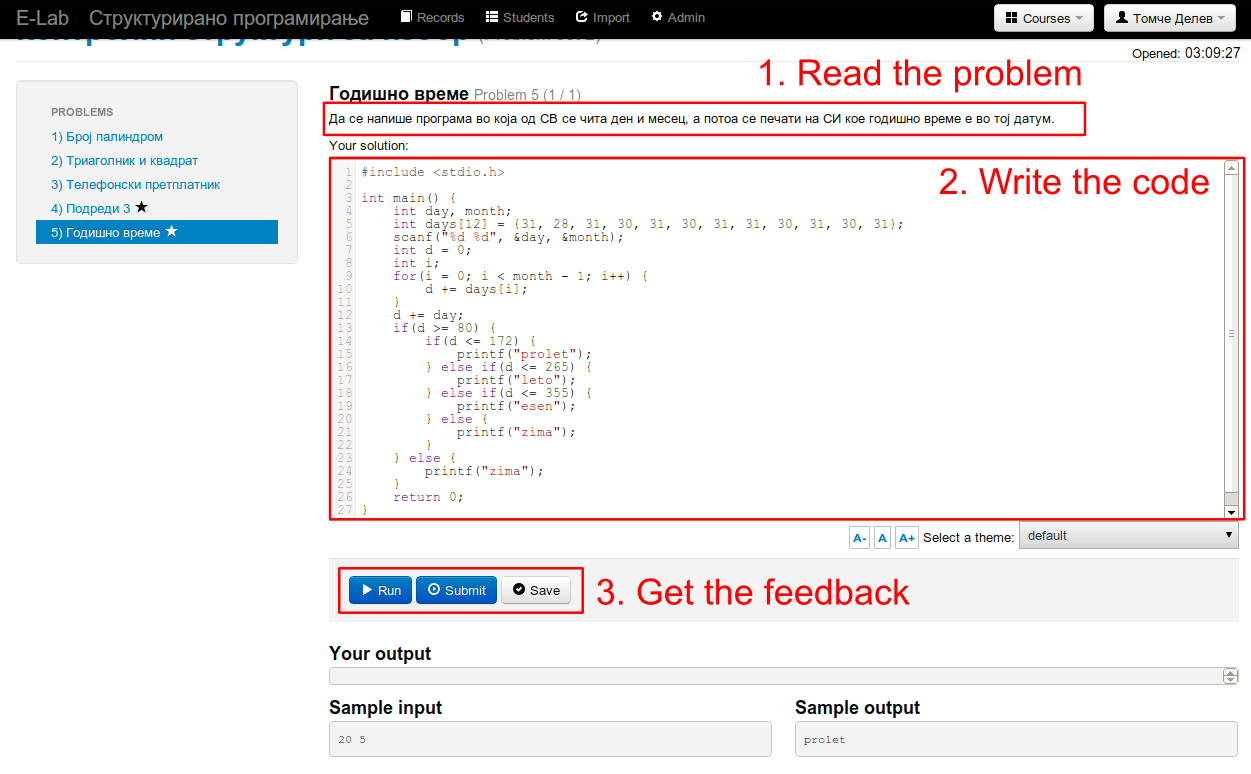
\includegraphics[width=.99\textwidth]{images/user_screen}
		\caption{The student screen trying to solve a problem.}
		\label{fig:student_screen}
	\end{figure}
\end{frame}

\begin{frame}{System architecture}
	\begin{figure}
	\centering
		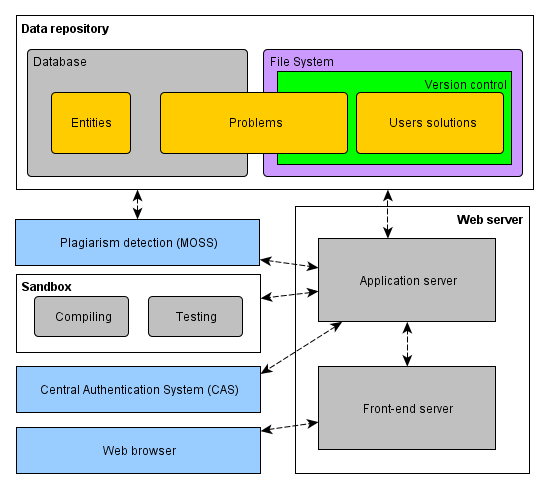
\includegraphics[width=.70\textwidth]{images/architecture}
		\caption{The E-Lab architecture.}
		\label{fig:architecture}
	\end{figure}
\end{frame}

\begin{frame}{Conclusion}
	\begin{itemize}[<+-| alert@+>]
	  \item Directly address the main organizational problems
	  \item Simplifying and improving the process of creating and managing
	  programming problems
	  \item Centralized repository (distributed)
	  \item E-Lab is not the silver bullet
	\end{itemize}
\end{frame}

\begin{frame}{Questions}{}
	\begin{center}
	\Large{
    \href{http://e-lab.finki.ukim.mk/}{\textbf{http://e-lab.finki.ukim.mk}}}
    \vfill
    \huge{Thank You}
    \vfill    
    \Huge{Questions?}
	
	\end{center}
\end{frame}

